\documentclass{tufte-handout}

\title{Propositional Probability III: Compilation\thanks{CS7470 Fall 2023: Foundations of Probabilistic Programming.}}


\newcommand{\varset}[0]{\mathcal{V}}

\author[]{Steven Holtzen\\s.holtzen@northeastern.edu}

%\date{28 March 2010} % without \date command, current date is supplied

%\geometry{showframe} % display margins for debugging page layout
\setcounter{secnumdepth}{1}

\usepackage{graphicx} % allow embedded images
  \setkeys{Gin}{width=\linewidth,totalheight=\textheight,keepaspectratio}
  \graphicspath{{graphics/}} % set of paths to search for images
\usepackage{amsmath,amssymb,amsthm}  % extended mathematics
\usepackage{booktabs} % book-quality tables
\usepackage{units}    % non-stacked fractions and better unit spacing
\usepackage{multicol} % multiple column layout facilities
\usepackage{lipsum}   % filler text
\usepackage{fancyvrb} % extended verbatim environments
  \fvset{fontsize=\normalsize}% default font size for fancy-verbatim environments
\usepackage{listings}
\usepackage{tikz}
\usepackage{mathpartir}
\usepackage{subcaption}
\usepackage{mdframed}
\usepackage{epigraph}
\usepackage{enumitem}
\usepackage{stmaryrd}

\usetikzlibrary{shapes.geometric}


\usepackage[ruled,linesnumbered]{algorithm2e}
\SetKwComment{Comment}{/* }{ */}
\newcommand{\indep}{\perp \!\!\! \perp}

\tikzset{
  treenode/.style = {shape=rectangle, rounded corners,
                     draw, align=center,
                     },
  root/.style     = {treenode, font=\Large, bottom color=red!30},
  env/.style      = {treenode, font=\ttfamily\normalsize},
  dummy/.style    = {circle,draw}
}

% tikz
\usetikzlibrary{patterns,calc,backgrounds}


% TIKZ
\tikzstyle{nnf}=[
  >=stealth,font=\small,auto,scale=0.7,every node/.style={scale=0.7}
]
\tikzstyle{extnode}=[
  draw,circle,inner sep=2pt,fill=white
]

\tikzstyle{leafnode}=[
  draw,fill=gray!20,inner sep=3.5pt
]
\tikzstyle{constnode}=[
  draw,fill=white,inner sep=3.5pt
]
\tikzstyle{label}=[
  fill=white,inner sep=2.5pt
]

\tikzstyle{acarrow}=[
    decoration={markings,mark=at position 1 with {\arrow[scale=0.6]{>}}},
    postaction={decorate},
    shorten >=0.4pt,
    >=latex,
    line width=0.1
]

\tikzstyle{bnarrow}=[
    decoration={markings,mark=at position 1 with {\arrow[scale=1.5]{>}}},
    postaction={decorate},
    shorten >=0.7pt,
    >=latex,
    line width=0.3
]
\tikzstyle{bayesnet}=[
  >=latex, thick, auto
]
\tikzstyle{bnnode}=[
  draw,ellipse,minimum size=7mm,inner sep=1pt,font=\small
]
\tikzstyle{cpt}=[
  font=\footnotesize
]

\tikzstyle{graph}=[
  >=stealth,font=\small,auto,scale=1,every node/.style={scale=1}
]
\tikzstyle{node}=[
  draw,circle,inner sep=3pt,fill=white
]

% BDDs

\tikzstyle{bdd}=[
  >=latex, thick, >=stealth, font=\small,auto,scale=0.9,every node/.style={scale=0.9}
]
\tikzstyle{bddnode}=[
  draw,circle,inner sep=0pt,fill=white,minimum size=5.5mm
]

\tikzstyle{bddtriangle}=[
  draw, regular polygon, regular polygon sides = 3,inner sep=1pt,fill=white,minimum size=5.5mm
]

\tikzstyle{highedge}=[
    line width=0.9
]
\tikzstyle{lowedge}=[
    line width=0.9,dotted
]
\tikzstyle{bddterminal}=[
  draw,fill=gray!20,inner sep=2.5pt, font=\small
]

\lstdefinestyle{compact}{
  \ttfamily\tiny
}


\usetikzlibrary{positioning}

\newtheorem{theorem}{Theorem}
\newtheorem{definition}{Definition}
\newtheorem{conjecture}{Conjecture}
\newtheorem{lemma}{Lemma}
\newtheorem{exercise}{Exercise}
\newtheorem{remark}{Remark}


\usepackage{xcolor}

\definecolor{codegreen}{rgb}{0,0.6,0}
\definecolor{codegray}{rgb}{0.5,0.5,0.5}
\definecolor{codepurple}{rgb}{0.58,0,0.82}
\definecolor{backcolour}{rgb}{0.95,0.95,0.92}

\lstdefinestyle{mystyle}{
    backgroundcolor=\color{backcolour},   
    commentstyle=\color{codegreen},
    keywordstyle=\color{magenta},
    numberstyle=\tiny\color{codegray},
    stringstyle=\color{codepurple},
    basicstyle=\ttfamily\footnotesize,
    breakatwhitespace=false,         
    breaklines=true,                 
    captionpos=b,                    
    keepspaces=true,                 
    numbers=left,                    
    numbersep=5pt,                  
    showspaces=false,                
    showstringspaces=false,
    showtabs=false,                  
    tabsize=2
}

\lstset{style=mystyle}

\newcommand{\defn}[1]{\textbf{#1}}
\newcommand{\dbracket}[1]{\left \llbracket {#1} \right \rrbracket}
\newcommand{\dist}[1]{\mathtt{Dist}(#1)}
\newcommand{\true}[0]{\texttt{true}}
\newcommand{\te}[0]{\texttt{e}}
\newcommand{\false}[0]{\texttt{false}}
\newcommand{\real}[0]{\mathbb{R}}
\newcommand{\rational}[0]{\mathbb{Q}}
\newcommand{\lebesgue}[0]{\mathbb{L}}
\newcommand{\eval}[0]{\mathrm{ev}}
\newcommand{\disc}[0]{\textsc{Disc}}
\newcommand{\borel}[0]{\mathcal{B}}
\newcommand{\ent}[0]{\mathbb{S}}
\newcommand{\prog}[0]{\texttt{p}}
\newcommand{\bool}[0]{\mathbb{B}}
\newcommand{\cont}[0]{\textsc{Cont}}
\newcommand{\prop}[0]{\textsc{Prop}}
\newcommand{\bdd}[0]{\textsc{Bdd}}
\newcommand{\robdd}[0]{\textsc{Robdd}}
\newcommand{\compiles}[0]{\rightsquigarrow}

\newcommand{\bddtriangle}[1]{
    \begin{tikzpicture}
    \node [bddtriangle] {#1};
    \end{tikzpicture}}
\newcommand{\bddtrue}[0]{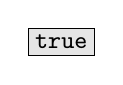
\begin{tikzpicture}
      \node [bddterminal] {$\true$};
    \end{tikzpicture}}
\newcommand{\bddfalse}[0]{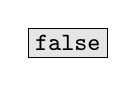
\begin{tikzpicture}
      \node [bddterminal] {$\false$};
    \end{tikzpicture}}


% Standardize command font styles and environments
\newcommand{\doccmd}[1]{\texttt{\textbackslash#1}}% command name -- adds backslash automatically
\newcommand{\docopt}[1]{\ensuremath{\langle}\textrm{\textit{#1}}\ensuremath{\rangle}}% optional command argument
\newcommand{\docarg}[1]{\textrm{\textit{#1}}}% (required) command argument
\newcommand{\docenv}[1]{\textsf{#1}}% environment name
\newcommand{\docpkg}[1]{\texttt{#1}}% package name
\newcommand{\doccls}[1]{\texttt{#1}}% document class name
\newcommand{\docclsopt}[1]{\texttt{#1}}% document class option name
\newenvironment{docspec}{\begin{quote}\noindent}{\end{quote}}% command specification environment



\begin{document}
\maketitle% this prints the handout title, author, and date
\begin{itemize}
  \item \defn{Goal:} to evaluate terms from \prop{} as efficiently as possible
  \item Last time we saw $(\pi, (\varphi, w)) \Downarrow^e v$. We observed that 
  it is efficient (i.e., polynomial in $|\varphi|$) if $\varphi$ has specific 
  forms: for instance, if it is a simple conjunction of variables. This time, we
  will see some more sophisticated evaluation strategies
\end{itemize}

\section{Memoization}
\begin{itemize}

  \item Consider the formula $(a \lor b) \land (c \lor d)$ and some $w$.

  
  \item Let's see a sketch of a derivation tree (where we elide $w$ and $\pi$
  for now):
  \begin{mathpar}
    \inferrule{
      \inferrule{
        \inferrule*[Left=($\star$)]{\dots}{c \lor d \Downarrow^e v_3}
        \and
        \inferrule{}{\false \Downarrow^e 0}
      }
      {(b \land (c \lor d)) \Downarrow^e v_1}
      \and
      \inferrule*[Right=($\star$)]{\dots}
      {(c \lor d)) \Downarrow^e v_2}
      }
    {((a \lor b) \land (c \lor d)) \Downarrow^e w(a)v_1 + w(\overline{a})v_2}
  \end{mathpar}

  \item \textbf{Observe}: both of the subtrees marked by $(\star)$ are \emph{identical}.
  We are wasting effort by re-deriving both. We should \emph{reuse} these derivations rather 
  than recomputing them.

  \item Now we will define a new reduction rule that memoizes previously computed results
  \marginnote{So far we've considered \emph{tree-like} proof-systems
  (also called \emph{Gentzen sequent calculus
  \citep{gentzen1969investigations}}): these are systems of deductions that
  describe trees, and cannot share sub-derivations.  There are more powerful
  DAG-like proof-systems that permit the reusing of subderivations. If you are
  interested in learning more about the power of various proof systems, check
  out \citet{beame2001propositional}}

  \item Shape of new relation: $(\rho, \texttt{p}) \Downarrow^m (v, \rho')$, where
  $\rho$ is a memoization table that maps \prop{} programs to probabilities:

  \begin{mathpar}
    \inferrule{}{(\pi, \rho, (\true, w)) \Downarrow^m (1, \rho)}
    \and
    \inferrule{}{(\pi, \rho, (\false, w)) \Downarrow^m (0, \rho)}
    \\
    \inferrule*[Left=\textsc{(Memo)}]{
    \rho(\varphi) = v \\
    }{(\pi, \rho, (\varphi, w)) \Downarrow^e (v, \rho)} 
    \\
    \inferrule*[Left=\textsc{(Split)}]{
    \varphi \notin \rho \\
    (\pi, \rho, (\varphi[\true/x], w)) \Downarrow^m (\rho', v_1) \\
    (\pi, \rho' \cup (\varphi[\true/x] \mapsto v_1), (\varphi[\false/x], w)) \Downarrow^m (\rho'',v_2) \\
    }{(x::\pi, \rho, (\varphi, w))  \Downarrow^m (\rho''\cup (\varphi[\false/x] \mapsto v_2), w(x)v_1 + w(\overline{x}) v_2)} \\
  \end{mathpar}

\end{itemize}

\subsection{Analysis of memoization}
\begin{itemize}
  \item What kinds of \prop{} programs does our new memoized reduction scale
  well on?
  \item For the purposes of analysis, it can be useful to give a
  \emph{cost-annotated} version of our rules that counts how many derivations
  were produced during runtime. This is fairly easy to do: we augment our relation 
  with an integer $n$ that accumulates the total runtime, so our new 
  relation is $(\pi, \rho, (\varphi, w)) \Downarrow (v, \rho', n)$:

  \begin{mathpar}
    \inferrule{}{(\pi, \rho, (\true, w)) \Downarrow^m (1, \rho, 1)}
    \and
    \inferrule{}{(\pi, \rho, (\false, w)) \Downarrow^m (0, \rho, 1)}
    \\
    \inferrule*[Left=\textsc{(Memo)}]{
    \rho(\varphi) = v \\
    }{(\pi, \rho, (\varphi, w)) \Downarrow^e (v, \rho, 1)} 
    \\
    \inferrule*[Left=\textsc{(Split)}]{
    \varphi \notin \rho \\
    (\pi, \rho, (\varphi[\true/x], w)) \Downarrow^m (\rho', v_1, n_1) \\
    (\pi, \rho' \cup (\varphi[\true/x] \mapsto v_1), (\varphi[\false/x], w)) \Downarrow^m (\rho'',v_2, n_2) \\
    }{(x::\pi, \rho, (\varphi, w))  \Downarrow^m (\rho''\cup (\varphi[\false/x] \mapsto v_2), w(x)v_1 + w(\overline{x}) v_2, n_1 + n_2 + 1)} \\
  \end{mathpar}

  \item Complexity in the \emph{elimination-width}, similar to variable
  elimination (won't get into that now...)

\end{itemize}

\section{Tractable runtimes}
\begin{itemize}
  \item \textbf{Problem}: evaluating probabilities is hard for \emph{arbitrary
  formulae}. What if we consider a \emph{restricted class} of formulae for which
  there exists a runtime semantics that \emph{guaranteed to be efficient in
  $|\varphi|$}? 
  % \marginnnote{This definition of tractable runtime is inspired by
  % \citet{darwiche2002knowledge}'s notion of a tractable language.}
  \begin{definition}[Tractable runtime]
    Let $p \Downarrow (v, n)$ be a cost-annotated big-step reduction relation
    for some program $p$ written in language $L$. We call $\Downarrow$
    a \defn{tractable runtime} if $n$ is polynomial in $(|\varphi|)$ for any program \texttt{p} 
    written in $L$.
  \end{definition}

  \item We need to define a notion of size for \prop{} programs. Intuitively, the size 
  simply counts how many syntactic constructs are utilized:
  \begin{mathpar}
    \inferrule{}{|\true| = 1} \and 
    \inferrule{}{|\false| = 1} \and 
    \inferrule{|\varphi| = n}{| \neg \varphi| = 1 + n} \and
    \inferrule{}{|x| = 1} \\ 
    \inferrule{|\alpha| = n_1 \and |\beta| = n_2}{|\alpha \land \beta| = 1 + |\alpha| + |\beta|}
  \end{mathpar}
  And so on similarly for other connectives.

  \item Observe: neither $\Downarrow^e$ nor $\Downarrow^m$ are tractable runtimes. \\
  \textbf{Exercise}: find a family of programs that witnesses this intractability for each 
  language.
  % Example family of programs that witnesses the intractability: exclusive-or programs\marginnote{
  %   Recall that exclusive-or, $a \oplus b$, is a connective that is true if and only if 
  %   $a$ and $b$ take on different values. It is macro-expressible in terms of $\lor$ and $\land$: 
  %   ($a \oplus b) = (a \land \neg b) \lor (\neg a \land b)$
  %   Also,
  %   observe that $(a \oplus b \oplus c)[a/\false] = \neg(b \oplus c)$
  % }

% \begin{lstlisting}[mathescape=true] ($\bigoplus_i^n x_i$, [$x_i \mapsto 0.5$])
% \end{lstlisting}

  \item Can we come up with a suitable restriction to \prop{} that guarantees 
  that $\Downarrow^e$ is a tractable runtime?

  \item \textbf{Idea}, our first tractable runtime: restrict propositional terms
  to be ``pre-split'' (or \emph{Shannon-expanded}). Call this language $\prop{}_{S}$:

\begin{lstlisting}[mathescape=true]
$\varphi_S, \alpha_S, \beta_S$ ::= true$_S$ | false$_S$ | $(x$_S$ \land \alpha_S) \lor (\neg x$_S$ \land \beta_S)$
$w_S ::= [x_S \mapsto \theta_x, \cdots]$
p$_S$ ::= ($\varphi_S, w_S$)
\end{lstlisting}
\item We define a cost-annotated enumeration relation $p_S \Downarrow^e (v, n)$ in a manner 
identical to \prop{} for \prop{}$_S$
\end{itemize}

\begin{theorem}
  Assume $p_S \Downarrow^e (v, n)$. Then, $n \le 1 + |p_S|$.
\end{theorem}

% 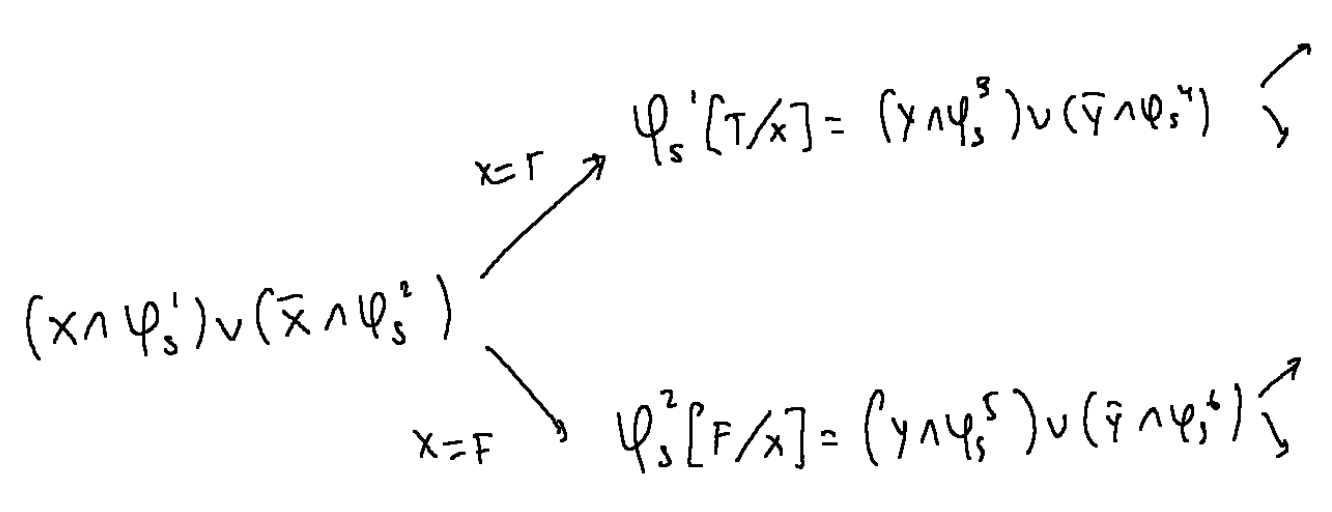
\includegraphics[width=250px]{searchtree.png}
\begin{proof}
  By structural induction on $(\varphi, w)$, inducting on $\varphi$. 
  Base cases are easy: $(\true, w) \Downarrow (1, 1) \le 1 + 1$.

  Now let's handle $((x \land \varphi_1) \lor (\neg x \land \varphi_2))$. 
  Assume by induction that $\varphi[\true/x] \Downarrow (v_1, n_1)$, $\varphi[\false/x] \Downarrow (v_2, n_2)$,
  and $n_1 \le 1 + |\varphi[\true/x]|$ and $n_2 \le 1 + |\varphi[\false/x]|$.

  Then, by applying the \textsc{(Split)} rule:
  \begin{mathpar}
  \inferrule{\varphi[\true/x] \Downarrow (v_1, n_1) \and \varphi[\false/x] \Downarrow (v_2, n_2)}
  {((x \land \varphi_1) \lor (\neg x
  \land \varphi_2)) \Downarrow^e (w(x) v_1 + w(\overline{x})v_2, 1 + n_1 + n_2)}
  \end{mathpar}
  Now we are done if we can conclude that $n_1 + n_2 \le |\varphi|$.
  Continuing:
  \begin{align}
   n_1 + n_2 &\le 1 + |\varphi[\true/x]| + 1 + |\varphi[\false/x]| & \text{by I.H.}\\
    & \le 1 + |\varphi_1[\true/x]| + 1 + |\varphi_2[\false/x]| & (\star) \\
    & \le 1 + |\varphi_1| + 1 + |\varphi_2| & (\star\star) \\
    & \le |(x \land \varphi_1) \lor (\neg x \land \varphi_2) & (\dagger)
  \end{align}
  where $(\star)$ follows from the definition of substitution, i.e. $\varphi[\true/x] = (x \land
  \varphi_1) \lor (\neg x \land \varphi_2)[\true/x] = \varphi_1[\true/x]$;
  
  $(\star\star)$ follows from a simple lemma:
  substitution can only reduce 
  the size of the formula, i.e. $|\varphi[v/x]| \le |\varphi|$ for any 
  variable $x$ and value $v$.

  $(\dagger)$ follows from the definition of $|\cdot|$.
\end{proof}

\subsection{Semantics-preserving translations}
\begin{itemize}
  \item \textbf{Idea}: we can give a semantics-preserving translation from an
  intractable language into a tractable one
  \item Why would we want to do that?
  \begin{itemize}
    \item Abstraction: just like we don't want all programmers to program in
    assembly, it's useful to identify good target languages
    \item Modular reasoning: We can separate our efficiency argument into 2 stages: 
    proving the target efficient, and proving the translation efficient (or characterizing 
    the efficiency of the translation)
  \end{itemize}
  \item Compilation from \prop{} to \prop{}$_S$: define a relation $\rightsquigarrow$ 
  that translates each term in each language while preserving semantics:

  \begin{figure}[h]
   \begin{mathpar}
    \inferrule{}{\true \compiles \true_S} 
    \and  
    \inferrule{}{\false \compiles \false_S} 
    \and
    \inferrule{}{x \compiles x_S} 
    \\
    \inferrule{x \text{ free in } \varphi \and
    \varphi[\true/x] \compiles \varphi_1 \and 
    \varphi[\false/x] \compiles \varphi_2
    }{\varphi \rightsquigarrow (x_S \land \varphi_1) \lor (\neg x_S \land \varphi_2)} 
  \end{mathpar}
   \caption{Compilation from \prop{} to \prop{}$_S$.}
   \label{fig:compile}
  \end{figure}

  \item We will want to prove this compilation correct by proving that it preserves denotation:
  \begin{definition}[Semantics preserving compilation]
    Let $L_1$ and $L_2$ be languages with semantic interpretations $\dbracket{\cdot}$
    with the same semantic domain.
    A compilation $\compiles$ from language $L_1$ to language $L_2$ is
    \defn{semantics-preserving} if, for any program $p_1$ written in $L_1$ 
    where $p_1 \compiles p_2$, it is the case that $\dbracket{p_1} = \dbracket{p_2}$.
  \end{definition}
  \begin{theorem}
    The compilation rules in Figure~\ref{fig:compile} are semantics-preserving.
  \end{theorem}
  \item In a seminal paper \citet{felleisen1990expressive} distinguished between
  different kinds of programming languages based on their supported syntactic features. He
  compared languages on the basis of \emph{expressivity}: whether or not it was
  possible to express all programs in one language in the other. 
  \item Here we consider a refinement of this notion to \emph{efficient
  expressiveness}, which captures whether or not an \emph{efficient} (i.e., polynomial-time)
  translation exists between two languages:
  \begin{definition}[Efficient expressiveness]
    A program $p_1$ written in language $L_1$ is \defn{efficiently expressible} 
    as a program $p_2$ written in language $L_2$ if
    there exists a polynomial-time semantics-preserving translation $p_1
    \rightsquigarrow p_2$. 
    We say language $L_1$ is \defn{efficiently expressible} as $L_2$, written $L_1 \sqsubseteq L_2$, 
    if all programs in $L_1$ are efficiently expressible as programs in $L_2$.
  \end{definition}

  \item Observe: $\prop_S$ is efficiently expressible as $\prop$, but not vice versa

  % \item Formally, \prop{}$_S$ is a sublangauge of \prop{} in the sense of
  % \citet{felleisen1990expressive}, so it can inherit its denotation and runtime
  % behavior. Here is a slightly informal definition (see \citet{felleisen1990expressive} for 
  % a more rigorous one):
  % \begin{definition}[Sublanguage]
  %   A language $L_1$ is a sublanguage of a super-language $L_2$ if (1) there
  %   exists an  (2) the semantics of every 
  % \end{definition}

  % \item Observe that every sublanguage is efficiently expressible as its super-language.


\end{itemize}

\section{Binary decision diagrams}
\begin{itemize}
  \item \textbf{Problem}: \prop$_S${} is not very expressive
  \item \textbf{Goal:} More expressive tractable languages
  \item What can we improve about \prop$_S$? Observe that there may be 
  \emph{repetitious sub-syntactic terms}, and we'd like to exploit those, just
  like we observed in our memoized reduction scheme
  \item How can we represent repetitious subterms syntactically? By changing our 
  syntax to permit \emph{directed acyclic graphs}!
  \item Syntax of \defn{binary decision diagram} (\bdd{}): a rooted binary directed acyclic graph 
  with two kinds of nodes:
  \begin{itemize}
    \item \emph{Choice nodes}, written \texttt{Ite($x, l, h$)}, where $x$ is a
    propositional variable (called the top variable), $l$ is an edge called the \emph{low edge}, and 
    $h$ is an edge called the \emph{high edge}
    \item \emph{Terminal nodes}, which are labeled $\true$ or $\false$.
  \end{itemize}
  \item The syntax of \bdd{} is given as graphical notation, for example:

  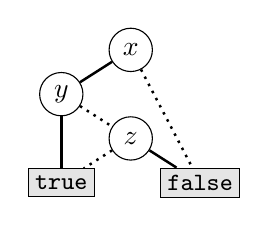
\begin{tikzpicture}
      
    \def\lvl{16pt}
    \node (inc) at (0bp,0bp) [bddnode] {$x$};

    \node (f1) at ($(inc) + (-25bp, -\lvl)$) [bddnode] {$y$};
    \node (f2) at ($(f1) + (25bp, -\lvl)$) [bddnode] {$z$};

    \node (vt) at ($(f2) + (-25bp, -\lvl)$) [bddterminal] {$\true$};

    \node (vf) at ($(f2) + (25bp, -\lvl)$) [bddterminal] {$\false$};
    \begin{scope}[on background layer]
      \draw [highedge] (inc) -- (f1);
      \draw [lowedge] (inc) -- (vf);

      \draw [lowedge] (f1) -- (f2);
      \draw [highedge] (f1) -- (vt);

      \draw [highedge] (f2) -- (vf);
      \draw [lowedge] (f2) -- (vt);
    \end{scope}

  \end{tikzpicture}

  Solid edges are high edges, dotted edges are low edges

  \item Semantics of \bdd{}:
  \begin{align*}
    \dbracket{
    \Gamma \vdash 
      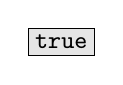
\begin{tikzpicture}
    \node (vt) [bddterminal] {$\true$};
    \end{tikzpicture}~} &= \dbracket{\Gamma}
    \\
    \dbracket{
    \Gamma \vdash 
      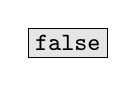
\begin{tikzpicture}
    \node (vt) [bddterminal] {$\false$};
    \end{tikzpicture}~} &= \emptyset
    \\
    \dbracket{
    \Gamma \vdash 
      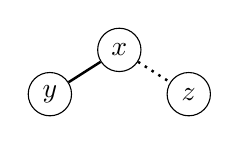
\begin{tikzpicture}
    \def\lvl{16pt}
    \node (x) at (0bp,0bp) [bddnode] {$x$};
    \node (t) at ($(x) + (-25bp, -\lvl)$) [bddnode] {$y$};
    \node (f) at ($(x) + (25bp, -\lvl)$) [bddnode] {$z$};
    \begin{scope}[on background layer]
      \draw [highedge] (x) -- (t);
      \draw [lowedge] (x) -- (f);
    \end{scope}
    \end{tikzpicture}~} &= \{ I \in \dbracket{y} \mid I(x) = \true \} \cup \{ I \in \dbracket{z} \mid I(x) = \false \}
  \end{align*}
\end{itemize}

% \section{Knowledge compilation}
% \begin{itemize}
%   \item \textbf{Goal}: give a compilation strategy from \prop{} to \bdd{}
% \end{itemize}



\bibliographystyle{plainnat}
\bibliography{../bib}

\end{document}